% Options for packages loaded elsewhere
\PassOptionsToPackage{unicode}{hyperref}
\PassOptionsToPackage{hyphens}{url}
\PassOptionsToPackage{dvipsnames,svgnames,x11names}{xcolor}
%
\documentclass[
  10pt,
  dvipsnames,enabledeprecatedfontcommands]{scrartcl}
\usepackage{amsmath,amssymb}
\usepackage{lmodern}
\usepackage{iftex}
\ifPDFTeX
  \usepackage[T1]{fontenc}
  \usepackage[utf8]{inputenc}
  \usepackage{textcomp} % provide euro and other symbols
\else % if luatex or xetex
  \usepackage{unicode-math}
  \defaultfontfeatures{Scale=MatchLowercase}
  \defaultfontfeatures[\rmfamily]{Ligatures=TeX,Scale=1}
\fi
% Use upquote if available, for straight quotes in verbatim environments
\IfFileExists{upquote.sty}{\usepackage{upquote}}{}
\IfFileExists{microtype.sty}{% use microtype if available
  \usepackage[]{microtype}
  \UseMicrotypeSet[protrusion]{basicmath} % disable protrusion for tt fonts
}{}
\usepackage{xcolor}
\usepackage{graphicx}
\makeatletter
\def\maxwidth{\ifdim\Gin@nat@width>\linewidth\linewidth\else\Gin@nat@width\fi}
\def\maxheight{\ifdim\Gin@nat@height>\textheight\textheight\else\Gin@nat@height\fi}
\makeatother
% Scale images if necessary, so that they will not overflow the page
% margins by default, and it is still possible to overwrite the defaults
% using explicit options in \includegraphics[width, height, ...]{}
\setkeys{Gin}{width=\maxwidth,height=\maxheight,keepaspectratio}
% Set default figure placement to htbp
\makeatletter
\def\fps@figure{htbp}
\makeatother
\setlength{\emergencystretch}{3em} % prevent overfull lines
\providecommand{\tightlist}{%
  \setlength{\itemsep}{0pt}\setlength{\parskip}{0pt}}
\setcounter{secnumdepth}{5}
\newlength{\cslhangindent}
\setlength{\cslhangindent}{1.5em}
\newlength{\csllabelwidth}
\setlength{\csllabelwidth}{3em}
\newlength{\cslentryspacingunit} % times entry-spacing
\setlength{\cslentryspacingunit}{\parskip}
\newenvironment{CSLReferences}[2] % #1 hanging-ident, #2 entry spacing
 {% don't indent paragraphs
  \setlength{\parindent}{0pt}
  % turn on hanging indent if param 1 is 1
  \ifodd #1
  \let\oldpar\par
  \def\par{\hangindent=\cslhangindent\oldpar}
  \fi
  % set entry spacing
  \setlength{\parskip}{#2\cslentryspacingunit}
 }%
 {}
\usepackage{calc}
\newcommand{\CSLBlock}[1]{#1\hfill\break}
\newcommand{\CSLLeftMargin}[1]{\parbox[t]{\csllabelwidth}{#1}}
\newcommand{\CSLRightInline}[1]{\parbox[t]{\linewidth - \csllabelwidth}{#1}\break}
\newcommand{\CSLIndent}[1]{\hspace{\cslhangindent}#1}
%\documentclass{article}

% %packages
 \usepackage{booktabs}
\usepackage{subcaption}
\usepackage{multirow}
\usepackage{colortbl}
\usepackage{graphicx}
\usepackage{longtable}
\usepackage{ragged2e}
\usepackage{etex}
%\usepackage{yfonts}
\usepackage{marvosym}
%\usepackage[notextcomp]{kpfonts}
\usepackage[scaled=0.86]{helvet}
\usepackage{nicefrac}
\newcommand*{\QED}{\hfill \footnotesize {\sc Q.e.d.}}
\usepackage{floatrow}
%\usepackage[titletoc]{appendix}
%\renewcommand\thesubsection{\Alph{subsection}}

\usepackage[textsize=footnotesize]{todonotes}
\newcommand{\inbook}[1]{\todo[color=gray!40]{#1}}
\newcommand{\mar}[1]{\todo[color=blue!40]{#1}}
\newcommand{\raf}[1]{\todo[color=olive!40]{#1}}
%\linespread{1.5}
\newcommand{\indep}{\!\perp \!\!\! \perp\!}


\setlength{\parindent}{10pt}
\setlength{\parskip}{1pt}


%language
\usepackage{times}
\usepackage{t1enc}
%\usepackage[utf8x]{inputenc}
%\usepackage[polish]{babel}
%\usepackage{polski}




%AMS
\usepackage{amsfonts}
\usepackage{amssymb}
\usepackage{amsthm}
\usepackage{amsmath}
\usepackage{mathtools}

\usepackage{geometry}
 \geometry{a4paper,left=35mm,top=20mm,}


%environments
\newtheorem{fact}{Fact}



%abbreviations
\newcommand{\ra}{\rangle}
\newcommand{\la}{\langle}
\newcommand{\n}{\neg}
\newcommand{\et}{\wedge}
\newcommand{\jt}{\rightarrow}
\newcommand{\ko}[1]{\forall  #1\,}
\newcommand{\ro}{\leftrightarrow}
\newcommand{\exi}[1]{\exists\, {_{#1}}}
\newcommand{\pr}[1]{\mathsf{P}(#1)}
\newcommand{\cost}{\mathsf{cost}}
\newcommand{\benefit}{\mathsf{benefit}}
\newcommand{\ut}{\mathsf{ut}}

\newcommand{\odds}{\mathsf{Odds}}
\newcommand{\ind}{\mathsf{Ind}}
\newcommand{\nf}[2]{\nicefrac{#1\,}{#2}}
\newcommand{\R}[1]{\texttt{#1}}
\newcommand{\prr}[1]{\mbox{$\mathtt{P}_{prior}(#1)$}}
\newcommand{\prp}[1]{\mbox{$\mathtt{P}_{posterior}(#1)$}}

\newcommand{\s}[1]{\mbox{$\mathsf{#1}$}}


\newtheorem{q}{\color{blue}Question}
\newtheorem{lemma}{Lemma}
\newtheorem{theorem}{Theorem}



%technical intermezzo
%---------------------

\newcommand{\intermezzoa}{
	\begin{minipage}[c]{13cm}
	\begin{center}\rule{10cm}{0.4pt}



	\tiny{\sc Optional Content Starts}
	
	\vspace{-1mm}
	
	\rule{10cm}{0.4pt}\end{center}
	\end{minipage}\nopagebreak 
	}


\newcommand{\intermezzob}{\nopagebreak 
	\begin{minipage}[c]{13cm}
	\begin{center}\rule{10cm}{0.4pt}

	\tiny{\sc Optional Content Ends}
	
	\vspace{-1mm}
	
	\rule{10cm}{0.4pt}\end{center}
	\end{minipage}
	}
%--------------------






















\newtheorem*{reply*}{Reply}
\usepackage{enumitem}
\newcommand{\question}[1]{\begin{enumerate}[resume,leftmargin=0cm,labelsep=0cm,align=left]
\item #1
\end{enumerate}}

\usepackage{float}

% \setbeamertemplate{blocks}[rounded][shadow=true]
% \setbeamertemplate{itemize items}[ball]
% \AtBeginPart{}
% \AtBeginSection{}
% \AtBeginSubsection{}
% \AtBeginSubsubsection{}
% \setlength{\emergencystretch}{0em}
% \setlength{\parskip}{0pt}






\usepackage[authoryear]{natbib}

%\bibliographystyle{apalike}



\usepackage{tikz}
\usetikzlibrary{positioning,shapes,arrows}

\ifLuaTeX
  \usepackage{selnolig}  % disable illegal ligatures
\fi
\IfFileExists{bookmark.sty}{\usepackage{bookmark}}{\usepackage{hyperref}}
\IfFileExists{xurl.sty}{\usepackage{xurl}}{} % add URL line breaks if available
\urlstyle{same} % disable monospaced font for URLs
\hypersetup{
  pdftitle={Gaps in the Evidence},
  pdfauthor={Marcello Di Bello; Rafal Urbaniak},
  colorlinks=true,
  linkcolor={Maroon},
  filecolor={Maroon},
  citecolor={Blue},
  urlcolor={blue},
  pdfcreator={LaTeX via pandoc}}

\title{Gaps in the Evidence}
\author{Marcello Di Bello\footnote{Arizona State University -
  \href{mailto:mdibello@asu.edu}{\nolinkurl{mdibello@asu.edu}}} \and Rafal
Urbaniak\footnote{University of Gdansk and Basis.ai}}
\date{May 09, 2023}

\begin{document}
\maketitle

\textbf{ROUGH DRAFT PLEASE DO NOT CITE OR DISTRIBUTE WITHOUT PERMISSION}

\paragraph*{Abstract}

The evidence presented in a trial may contain gaps. These gaps can be
manifest, for example, when it is common knowledge among the litigants
that a body of relevant information was lost or could not be retrieved.
Gaps in the evidence can also be conjectural, for example, when
information that one would reasonably expect to see in a case is not
presented. Should gaps in the evidence matter for trial decision-making?
How can appropriate remedies be formulated to compensate the litigant
negatively affected by gaps in the evidence? Using a probabilistic
model, we show that gaps in the evidence can themselves constitute
relevant evidence. After considering some examples in the case law, we
argue that the formulation of remedies should take into account
epistemic and non-epistemic considerations. Two questions are important:
whether the missing evidence, if added, would have enhanced the accuracy
of the decision-making process, and second, whether gaps exist for
fortuitous or non-fortuitous reasons. These questions partly overlap
with the legal framework for handling gaps in the evidence which
emphasizes the question of prejudice and bad faith intent.

\tableofcontents

\hypertarget{introduction}{%
\section{Introduction}\label{introduction}}

This is uncontroversial about trial decision-making: disputes about
matters of fact should be adjudicated in light of the evidence presented
by the litigants. Suppose a plaintiff sues a shop owner because of an
injury that occurred in the shop. The floor was slippery. The plaintiff
tripped and fell. They had a concussion. They seek compensation for
damages. This is the plaintiff's story. The shop owner disagrees. The
plaintiff did fall and had a concussion---this is undisputed---but not
because of the slippery floor. Plaintiff and defendant are disagreeing
about a question of fact. What happened, exactly, when the plaintiff
tripped and fell? Evidence must be presented by the litigants to resolve
the dispute.

But there is a complication. Suppose the shop had cameras inside. When
the plaintiff tripped and fell, the camera recorded what happened. The
recording, if accessible, could unequivocally tell what happened. For
some reason, however, the camera recording of that specific incident had
gone missing. And, unfortunately, that day at that time no one else was
in the shop. So there isn't much other evidence that could be gathered,
except conflicting testimonies by the plaintiff and defendant. Merely
based on the available evidence, then, the plaintiff would have a weak
case and lose the lawsuit.

This outcome would be, in some important way, unsatisfactory. Why was
the recording missing? The shop owner might have deleted it, fearing
that the customer could sue them. If so, should the case be resolved in
favor of the plaintiff even though the available evidence does not tip
in their favor? Perhaps so. What if the recording was deleted by
accident? Our intuitions might waver. Setting aside how the case should
be decided, the upshot here is this. For one thing, the evidence
presented by the parties should guide trial decisions. For another, the
fact that some evidence was \textit{not} presented should also---in some
circumstances---be considered evidence and thus guide trial decisions.
To examine what these circumstances might be is the task of this paper.
We call this the problem of gaps in the evidence or the problem of
missing evidence.

Legal systems of adjudication contain rules for handling gaps in the
evidence. These rules are elaborate, subtle, intricate. We are not
cataloging these rules, nor offering a comparative study of how
different systems of adjudication address the problem of gaps. Our aim
here is modest---that is, to map out the conceptual terrain.\footnote{On
  the importance of `comprehensive evidence' for epistemic warrant, see
  Haack (1995). For the authors' earlier discussions on incomplete
  evidence, see Di Bello (2013) and Urbaniak (2018).} The plan is as
follows. Contrary to existing claims in the literature, Section
\ref{sec:missing-evidence-evidence} shows that missing evidence can be
relevant evidence. Section \ref{sec:legal-framework} sketches how the
law handles missing evidence in a few paradigmatic examples. We will
draw from the case law of the United States, but we hope our discussion
can have a more general interest. Section
\ref{sec:prejudice-reliability} examines more closely the question of
prejudice. The case law tends to focus on whether the missing evidence
could have made a difference to the verdict. We think, instead, that the
question whether the missing evidence could have enhanced the accuracy
of the decision-making process is more fundamental. This focus on
accuracy need not be in tension with legal practice, however. Section
\ref{sec:remedies} examine remedies for missing evidence, in particular,
how epistemic and policy considerations can guide the formulation of
these remedies. Finally, Section \ref{sec:end} identifies two central
questions that should inform responses to missing evidence: first,
whether the missing evidence would have enhanced the accuracy of the
decision-making process; and second, whether the evidence is missing for
fortuitous or non-fortuitous reasons.

\hypertarget{missing-evidence-is-evidence}{%
\section{Missing evidence is
evidence}\label{missing-evidence-is-evidence}}

\label{sec:missing-evidence-evidence}

That some evidence had gone missing---say, that the recording of the
customer's fall had gone missing---is itself a piece of information. It
can be treated as evidence, that is, evidence that (some other) evidence
is missing. The question is whether this evidence-missing evidence is
relevant for adjudicating a dispute about a matter of fact. We will see
that the answer is in a wide range of cases surely positive.

\hypertarget{balance-of-missing-and-available-evidence}{%
\subsection{Balance of missing and available
evidence}\label{balance-of-missing-and-available-evidence}}

If the fact that evidence is missing is itself treated as an item of
evidence, this information can contribute to the overall balance of the
evidence. We borrow the expression `balance of evidence' from J.M.
Keynes (1921) to describe the outcome of weighing evidence for and
against a certain hypothesis of interest.\footnote{For an extended
  discussion of balance as opposed to weight of evidence, see Nance
  (2016).} In general terms, the model we have in mind is the following.
Suppose the balance of the evidence is quantified using a probability
measure, such as that probability that the defendant is liable \(L\)
given the available evidence \(E_a\), or written in symbols,
\(\pr{L \vert E_a}\). This account is incomplete, however. The balance
of evidence should also comprise facts about missing evidence \(E_m\).
So, following a suggestion by Kaye (1986), a more complete account would
be the probability that the defendant is liable \(L\) given the
available evidence \(E_a\) as well as facts about missing evidence
\(E_m\), or in other words, \(\pr{L \vert E_a \wedge E_m}\). Once such a
probability can be assessed, it can be used further down the path of
evidential reasoning. Unfortunately, Kaye does not provide a method for
how this task should be carried out, leaving open the possibility that
\(\pr{L \vert E_a}\) and \(\pr{L \vert E_a \wedge E_m}\) turn out to be
the same.

To make progress here, the key question is whether this evidence-missing
evidence \(E_m\) is relevant evidence. Relevance is traditionally
defined as the conjunction of (a) probative value and (b) materiality.
Rule 401 of the Federal Rules of Evidence reads:

\begin{quote}
Evidence is relevant if: (a) it has any tendency to make a fact more or less probable than it would be without the evidence; and (b) the fact is of consequence in determining the action.
\end{quote}

\noindent So the question is whether \(\pr{L \vert E_a}\) and
\(\pr{L \vert E_a \wedge E_m}\) can differ, or more generally whether
\(\pr{H \vert E_a}\) and \(\pr{H \vert E_a \wedge E_m}\) can differ,
where \(H\) is any material hypothesis.

The problem with missing evidence is that its content is unknown. For
all we know, the video recording could have shown that the customer
tripped and fell because of the slippery floor or for some other reason.
Without knowing its content---some might argue---the relevance of
missing evidence is essentially null. The following passage from Hamer
(2012) makes this point:

\begin{quote}
\dots if the evidence is missing it cannot be known which way it points.
It appears equally possible that the missing evidence would confirm the current factual conclusion as contradict it. The competing possibilities cancel each other out. There is no warrant for the assumption that the missing evidence will point one way rather than the other. [p. 139]
\end{quote}

\noindent This argument has some plausibility. But there are good
reasons to question it. Indeed, missing evidence can point in two
directions---in favor or against the defendant---but evidence does not
exist in a vacuum. When it is part of a known causal structure,
plausible inferences can be drawn about which way it \emph{would have
pointed} even without knowing which ways it does point. The opposite
directions the missing evidence could have pointed need not always
cancel each other out. The plausibility of Hamer's argument hinges on
the assumption that facts about missing evidence occurred at random.
When this assumption does not hold, facts about missing evidence are
more likely on some scenarios than on others. The intuition that the
direction in which missing evidence could point should balance out no
longer works. We will make this point precise using a probabilistic
model of missing evidence.

Before we move on, however, we should note that one need not subscribe
to a probabilistic model of the balance of evidence. Whatever one's
model, it will need to accommodate the evidential value of missing
evidence. Consider, for the sake of illustration, another popular
account of the balance of evidence: the theory of relative plausibility
by Pardo \& Allen (2008). On this account, the competing hypotheses
under consideration in a trial---say the story put forward by the
defense and the story put forward by the plaintiff---should be evaluated
in light of how well they explain the evidence. So long as the evidence
comprises both the available evidence and facts about missing evidence,
the competing hypotheses should be evaluated in light of how well they
explain the overall evidence, \(E_a\wedge E_m\). There is no reason why
facts about missing evidence could not themselves be the target of an
explanation. So, on this account, the hypothesis that better explains
the available evidence as well as facts about missing evidence would be
explanatory superior to its rival. The exact details of this analysis
should be worked out and we do not take up this task here. In what
follows, instead, we rely on the probabilistic account because it can
make precise the relevance of missing evidence.

\hypertarget{bayesian-network-model}{%
\subsection{Bayesian network model}\label{bayesian-network-model}}

To substantiate the claim that missing evidence can be relevant,
consider more closely the somewhat simplistic but illustrative trip and
fall case. The underlying causal structure can be modeled using a
Bayesian network that comprises a graphical, qualitative part and a
numerical part.\footnote{For an illustration of how Bayesian network can
  be used to model evidence in legal cases, see Fenton, Neil, \& Lagnado
  (2013).} The graphical part consists of variable nodes, their values,
and arrows between the nodes (see Figure \ref{fig:dag-missing-video}).
The \textit{nodes} stand for event variables, such as the slippery floor
(\textsf{Slippery}) and the defendant's attempt to destroy the recording
(\textsf{Interference}), or evidence variables, such as the defendant's
testimony that they fell because of the slippery floor and the video
recording (\textsf{Video}). Each variable can take two or more
\textit{values}. The video variable can take three values since the
recording could show the floor was safe (\textsf{Video}=\textsf{safe}),
dangerous (\textsf{Video}=\textsf{dangerous}) or the video itself could
be missing (\textsf{Video}=\textsf{missing}). The other variables will
take two values, say the floor was slippery (\textsf{Slippery}=
\textsf{yes}) or not (\textsf{Slippery}= \textsf{no}), the interference
happened (\textsf{Interference}=\textsf{yes}) or not
(\textsf{Interference}=\textsf{yes}), and so on. Finally, the
\textit{arrows} represent relations of causal influence between variable
nodes: whether the floor was slippery or not affects the content of the
video; it also affects whether the customer fell or not; and so on.

\begin{figure}[t]
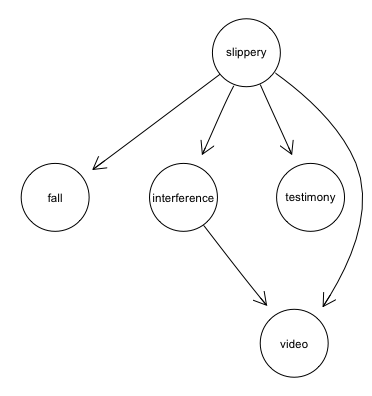
\includegraphics[width=5cm]{slippery-dag.png}
\caption{A direct acyclic graph for the trip and fall case.}
\label{fig:dag-missing-video}
\end{figure}

These qualitative relations of causal influence can be quantified using
probabilities. This is the numerical part of the Bayesian network,
usually in the form of probability tables (see Table
\ref{table:prob-missing-video}). Say, if the floor was slippery it is
twice as likely that one would fall compared to when the floor was not
slippery. Updating the network with the information that the customer
fell makes the hypothesis that the floor was actually slippery more
likely: the probability of the hypothesis goes from a stipulated 10\% to
16\% in our simulation. This accords with our intuitions. Consider now
the possibility of interference. Say, if the floor was slippery, it is
twice as likely that there would an interference by the owner than when
the floor was not slippery. In addition, if there was an interference by
the owner, it is extremely likely the video would be missing, even
though the video could also be missing because of other, more fortuitous
circumstances. Assume the likelihood the video would be missing under
the interference hypothesis is nine times more likely than under the
non-interference hypothesis. Given this 9:1 ratio, updating the network
with the information that the video is missing makes the hypothesis that
the floor was slippery even more likely: its probability goes from 16\%
to 26\%.

\begin{table}
\begin{tabular}{r | cc cc}
& \multicolumn{4}{c}{P(Slippery)}\\
                     & \multicolumn{2}{c}{Slippery=yes}  & \multicolumn{2}{c}{Slippery =no}  \\
                      & \multicolumn{2}{c}{1/10}          & \multicolumn{2}{c}{9/10}      \\
\hline
& \multicolumn{4}{c}{P(Fall | Slippery)}\\
                     & \multicolumn{2}{c}{Slippery=yes}  & \multicolumn{2}{c}{Slippery =no}  \\
Fall=yes             &   \multicolumn{2}{c}{2/3}          &  \multicolumn{2}{c}{1/3}        \\
Fall=no              &   \multicolumn{2}{c}{1/3}          & \multicolumn{2}{c}{2/3}        \\
\hline
& \multicolumn{4}{c}{P(Interference | Slippery)}\\
                     & \multicolumn{2}{c}{Slippery=yes}& \multicolumn{2}{c}{Slippery =no}  \\
Interference = yes    &  \multicolumn{2}{c}{2/3}          & \multicolumn{2}{c}{1/3}             \\
Interference = no     & \multicolumn{2}{c}{1/3}           & \multicolumn{2}{c}{2/3}           \\
\hline
& \multicolumn{4}{c}{P(Video | Slippery, Inference) - \textit{first scenario}}\\
                     & \multicolumn{2}{c}{slippery=yes}   & \multicolumn{2}{c}{Slippery =no}  \\
                    & Interference=yes & Interference=no & Interference=yes &Interference =no\\   
Video = safe         &  0               &       0         &           0         &        9/10 `    \\ 
Video = danger       &  0               &       9/10      &           0         &        0         \\ 
Video = missing      &  1               &       1/10      &           1         &        1/10       \\ 
\hline
& \multicolumn{4}{c}{P(Video | Slippery, Inference) - \textit{second scenario}}\\
                     & \multicolumn{2}{c}{slippery=yes}   & \multicolumn{2}{c}{Slippery =no}  \\
                     & Interference=yes & Interference=no & Interference=yes &Interference =no\\   
Video = safe         &  0               &       0         &           0         &        6/10      \\ 
Video = danger       &  0               &       6/10      &           0         &        0         \\ 
Video = missing      &  1               &       4/10      &           1         &        4/10       \\ 
\end{tabular}
\caption{Plausible probabilities for the Bayesian network about the trip and fall case.}
\label{table:prob-missing-video}
\end{table}

These numbers are purely illustrative. Changing the ratio to 6:4---that
is, the video could be missing for fortuitous reasons in 40\% of
cases---weakens the inference from the missing video to the conclusion
that the floor was slippery. The hypothesis that the floor was slippery
would now change from 16\% to 22\% probability. But, no matter the exact
numbers, the missing video \textit{is} relevant evidence---or more
precisely, the fact that the video recording is missing is itself
relevant information. Taking into account that the recording is missing
increases the probability that the floor was slippery. This conclusion
holds even though the content of the video remains unknown. The only
case in which the missing video would have null value is if there is no
relation between the slippery floor and the owner's interference---that
is, if it was just as likely that the owner would attempt to remove the
recording when the floor was slippery than when it was not.

\hypertarget{objections}{%
\subsection{Objections}\label{objections}}

The claim we are putting forward is that facts about missing evidence
can---as in the trip and fall case---be relevant evidence. Some might
resist this conclusion for the following reason. Cases of missing
evidence do not usually contain direct evidence indicating that the fact
of missing evidence is itself relevant. This is the very question that
needs to be addressed and its answer cannot be presupposed from the
outset. For example, even if the video recording is missing, this cannot
be evidence that the owner attempted to destroy or alter the recording.
Absent direct evidence that the owner attempted or had reasons to
destroy the recording, the owner should be given the benefit of the
doubt.

But, even though there is no direct evidence that the owner attempted to
destroy the video, the fact of missing evidence is itself evidence that
the owner attempted to destroy the video. This falls out of the Bayesian
network and the probability assumptions embedded in it. One might insist
that even if, statistically speaking, whenever a recording is missing,
it is more likely due to a deliberate action than an accident, this
statistical regularity does not apply to the instant case. In fact,
statistical regularities cannot tell us about individual actions. This
observation is hard to make sense of, however. For information that a
witness saw the defendant from far away is routinely used to weaken the
credibility of witness identifications. This weakening rests on
statistical regularities about decreasing levels of reliability in
witness identifications as distance increases. But, perhaps, the
objection underscore a different point. Available evidence can be
scrutinized: a testimony can be questioned, challenged, tested during
cross-examination. Missing evidence---or so the argument goes---cannot
be scrutinized: it is an inert fact from which we cannot know anything
more. So, facts about missing evidence cannot be given the same status
as available evidence.

This line of questioning is well taken, but the distinction drawn here
is more of a quantitative than a qualitative type. Existing
psychological research challenges the assumption that cross-examination,
at least as currently practiced, is an effective method for
distinguishing between reliable and unreliable evidence: questions asked
in an adversarial setting under stressful circumstances may result in a
biased assessment of the reliability of the witness testimony (Epstein,
2007). Furthermore, in principle there is no reason why one couldn't
scrutinize the evidence about the missing evidence itself, say by
questioning the shop's personnel about the data-management practices.
This line of questioning could help to see how likely it is that the
evidence went missing due to negligence rather than to ill will.

Still, we concede that facts about missing evidence often involve a
greater degree of uncertainty---and ultimately, we think that such sort
of uncertainty could be better modeled in terms of higher-order
probabilities. Every item of evidence is characterized by at least two
levels of uncertainty. There is a first-order uncertainty about the
hypothesis that the evidence is intended to support, for example, it is
more or less likely that a hypothesis is true given the evidence. In
addition, there is uncertainty about the first-order uncertainty itself,
for example, it is more or less likely that it is more or less likely
that the hypothesis is true given the evidence. We think that facts
about missing evidence usually carry a higher second-order uncertainty,
compared to available evidence. We do not pursue this analysis here,
however.

The fact that often there is more uncertainty about missing evidence
does not undermine the claim that the missing evidence can be relevant,
as we have shown. There may be overriding, non-epistemic reasons to
ignore it, but its epistemic value is not necessarily null. To better
understand the interplay between epistemological and non-epistemological
considerations, we now turn to how the law handles cases of missing
evidence. This is our next topic.

\hypertarget{legal-framework}{%
\section{Legal framework}\label{legal-framework}}

\label{sec:legal-framework}

The legal framework for dealing with missing evidence is informed by a
number of questions. They pertain to the would-be-relevance of the
missing evidence, its prejudicial effects, and the remedies that can be
applied. Considerations about why the evidence is missing are also
important.

\begin{itemize}
\item[] \textit{Would-be-relevance} - Would the missing evidence if presented be relevant?
\item[] \textit{Prejudice} - Could the missing evidence make a difference to the decision?
\item[] \textit{Circumstances} - Why is the evidence missing? Was it an accident or misconduct? Did one of the parties have a duty to preserve the missing evidence?
\item[] \textit{Remedy} - What remedies should be granted to the litigant disadvantaged 
by the missing evidence?
\end{itemize}

\noindent The context here is that one of the litigants complains about
missing evidence and asks for a remedy, say a missing evidence
instruction, a sanction against the other party, retrial. The
complaining party should make a case that the missing evidence is
relevant and prejudicial, and also that a remedy must be granted that
would be appropriate to the circumstances. These complaints are made
because the other party failed to comply with a request to disclose
information, documents and witnesses relevant to the case.\footnote{See,
  for example, Rule 37 (Failure to Make Disclosures or to Cooperate in
  Discovery; Sanctions) of Federal Rules of Civil Procedures and Rule 16
  (Discovery and Inspection) of Federal Rules of Criminal Procedure.}

\hypertarget{relevance-and-prejudice}{%
\subsection{Relevance and prejudice}\label{relevance-and-prejudice}}

At first blush, the first two questions can be understood as forming a
flowchart. If the missing evidence is not relevant, the question of
prejudice does not arise. If the evidence is not prejudicial, the other
questions---especially the question of what remedies should be
granted---does not arise. But this interpretation is overly rigid and
needlessly algorithmic. These questions are better considered
holistically. An understanding of the circumstances that caused the
evidence to be missing will help to discern whether the evidence is
relevant or prejudicial, and thus also select the appropriate remedy. It
is helpful, though, for analytical clarity, to consider the first two
questions separately.

The question of relevance here must be understood in a peculiar manner.
As noted before, relevance is traditionally defined as the combination
of (a) probative value and (b) materiality. But the question of
relevance for missing evidence in the legal framework is not a standard
question of relevance. It requires a judgment of \textit{would-be}
relevance. Missing evidence is evidence whose content is generally
unknown. It could favor one side or the other side, say it could be
incriminating or exculpatory. If the content of the missing evidence
were known, the evidence would not be missing in the full sense. So, in
order to meet the would-be-relevance test, the missing
evidence---however its content turns out to be exactly---should
strengthen or weaken the case of one of the litigants. More precisely,
the party complaining about missing evidence must demonstrate

\begin{quote}
``a relationship between the requested evidence and the issues in the
case, and there must exist a reasonable indication that the requested
evidence will either lead to other admissible evidence, assist the
defendant in the preparation of witnesses or in corroborating testimony,
or be useful as impeachment or rebuttal evidence.'' United States v.
Curtis , 755 A.2d 1011, 1014--15 (D.C. 2000), cited in Buchanan v.
United States, 165 A.3d 297, 304 (D.C. 2017).
\end{quote}

\noindent And to put the requirement more clearly in terms of altering
the balance of the available evidence:

\begin{quote}
``The defense must show more than that the item bears some abstract
logical relationship to the issues in the case. There must be some
indication that \ldots{} the item would enable the defendant
significantly to alter the quantum of proof in his favor.'' United
States v. Jordan , 316 F.3d 1215, 1251 (11th Cir. 2003).
\end{quote}

\noindent Short of that, any litigation about missing evidence should
not even begin. The bar is high.

It might not always be clear whether the would-be-relevance test is met.
For example, suppose the defendant is charged with illegal possession of
firearm. The police legally searched the defendant's vehicle and found a
firearm. The defendant had no permit. The police searches the rest of
the car and finds a backpack, but does not retain all the items in the
backpack: keys, pieces of paper, trash. The defense complains that the
evidence is incomplete: information about the contents of the backpack
is missing. On one interpretation, the missing evidence seems
irrelevant. The evidence available shows conclusively that the defendant
was carrying a firearm without a permit. The exact content of the
backpack does not make any difference.\footnote{Howard v. United States
  - No.~18-CF-157 District of Columbia Court of Appeals Link to case:
  \url{https://www.dccourts.gov/sites/default/files/2020-11/Howard\%20v\%20United\%20States\%2018-CF-157.pdf}}

But the party adversely affected by the missing evidence---the defendant
here---might object. What if an item in the backpack---say, the
keys---could have indicated the backpack was not the defendant's?

\begin{quote}
Counsel for appellant \ldots{} {[}suggested{]} that even if the defense
team had been unable to locate the owner of the key, they could have
tried the key at Howard's dwelling and demonstrated that it was not his.
In other words, even if the defendant could not point the finger at any
particular third party, he could present a theory that the backpack was
shared. (Howard v. United States - No.~18-CF-157 District of Columbia
Court of Appeals, p.~15)
\end{quote}

\noindent So the keys could be exculpatory evidence. If they did not
belong to the defendant, the backpack did not either, and neither did
the firearm---or so the defense could argue. Perhaps this argument is
sufficient to alter the balance of evidence and create a reasonable
doubt. In this way, however, any missing piece of information---given a
broad enough interpretation---can pass the would-be relevance test and
potentially alter the balance of the existing evidence.

The response of the court to the defendant's argument is worth citing in
full:

\begin{quote}
``Appellant's argument is based entirely on speculation. It is, of
course, equally plausible that the key was Howard's and that it would
have provided additional evidence of his guilt. And though identifying
the backpack as Howard's was important, the weapon was found underneath
appellant's seat after officers watched him lean forward and then sit
back up when he saw that the car was being pulled over. \ldots{} the
exculpatory value of the key was wholly speculative \ldots{} there was
additional evidence outside of the backpack linking the gun to Howard,
and \ldots{} other evidence indicated that the backpack and its contents
were indeed his'' (ibid, p.~17)
\end{quote}

\noindent How should we interpret the Court's reasoning? Perhaps, we
need not split hair about the would-be-relevance test. Granted, the
keys---under a plausible interpretation---could be relevant exculpatory
evidence. But what matters is whether the missing (relevant) evidence
could make a difference for the decision, in light of all other evidence
available. If it cannot---even interpreted in the light most favorable
to one of the parties---the question whether we should worry about the
missing evidence is moot. In other words, the question of relevance
becomes moot \emph{absent prejudice}. So the first two questions of
relevance and prejudice boil down to the question of prejudice: whether
the missing evidence could tilt the scale in favor of the defendant so
significantly that the verdict would turn around.

\hypertarget{circumstances-and-remedies}{%
\subsection{Circumstances and
remedies}\label{circumstances-and-remedies}}

Let's now tackle the question of remedies. This question offers great
latitude. An extreme remedy would be this: if the missing evidence is
detrimental to the accused, the case should be dismissed. This remedy is
excessive: it will create a perverse incentive for defendants to destroy
evidence in their favor. The absence of evidence that could be in favor
of the defendant would be enough to dismiss the accusation. Instead of
presenting exculpatory evidence to be tested via cross-examination,
defendants would prefer to destroy it. They would then argue they were
prejudiced and should win the case. This arrangement makes little sense.
Alternatively, such a remedy could apply only provided the party
bringing the accusation was responsible for destroying the evidence
favoring the defendant.

Remedies can also apply at the level of how the evidence is assessed,
not directly to decisions. So, for example, the remedy could be this:
the party responsible for the missing evidence and that attempted to
benefit from this fact should have their case weakened by a quantum of
evidential force proportionate to the extent to which the party sought
to benefit by causing the gap. There are other possible formulations,
for example, an adverse jury instruction to presume a fact obtained,
where the presumed fact weakens the case of the party that, in bad
faith, contributed to the destruction of the evidence.

Another approach would be to initiate a separate litigation for missing
evidence. This might be more appropriate in criminal than civil cases.
To penalize criminal defendants with adverse jury instructions because
they destroyed evidence may clash with other well-established rights
defendants have, such as the right to be presumed innocent until proven
guilty. At the same time, destruction of incriminating evidence must be
negatively sanctioned. To this end, destruction or tainting of evidence
relevant for criminal litigation can count as a wrongdoing in itself
which can be litigated in a separate trial. This should provide the
right incentive for people not to destroy evidence.

This survey of possibilities is not exhaustive. To get a sense for the
broader array of remedies available, here is an excerpt from N.Y. Crim.
Proc. Law § 245.80, 2 (Available remedies or sanctions):

\begin{quote}
For failure to comply with any discovery order imposed or issued
pursuant to this article, the court may make a further order for
discovery, grant a continuance, order that a hearing be reopened, order
that a witness be called or recalled, instruct the jury that it may draw
an adverse inference regarding the non-compliance, preclude or strike a
witness's testimony or a portion of a witness's testimony, admit or
exclude evidence, order a mistrial, order the dismissal of all or some
of the charges provided that, after considering all other remedies,
dismissal is appropriate and proportionate to the prejudice suffered by
the party entitled to disclosure, or make such other order as it deems
just under the circumstances; except that any sanction against the
defendant shall comport with the defendant's constitutional right to
present a defense, and precluding a defense witness from testifying
shall be permissible only upon a finding that the defendant's failure to
comply with the discovery obligation or order was willful and motivated
by a desire to obtain a tactical advantage.
\end{quote}

\hypertarget{bad-faith-and-adverse-jury-instruction}{%
\subsection{Bad faith and adverse jury
instruction}\label{bad-faith-and-adverse-jury-instruction}}

Given the wide range of possibilities, it is helpful to focus on a
specific version of remedies that is quite paradigmatic: an adverse jury
instruction against a party granted because of the party's bad faith.
Often, if one of the parties destroyed evidence in bad faith, an adverse
jury instruction is warranted against that party---say, presuming that
the missing evidence was in fact unfavorable to that party.

Consider a more elaborate version of the trip and fall case at the start
of this paper.\footnote{Details of the case are as follows: Decker v.
  Target Corp, Case No.~1:16-cv-00171-JNP-BCW, Filed 10/10/2018} An
accident occurs at Target, a chain of department stores in the United
States. The customer slips, falls and gets injured in a Target store
because of a flatbed, possibly left unattended. The customer suffers
serious injury and is transported to a hospital. The customer sues
Target and seeks to recover damages. However, video surveillance footage
is only preserved in part. The rest is destroyed. It is impossible to
reconstruct what happened before the incident.\footnote{The incident
  occurred on December 26, 2015, at the Target store located in
  Riverdale, Utah: ``Caryl Jean Decker was shopping when she tripped on
  a flatbed stocking cart and fell onto the floor, suffering serious
  injury. Mrs.~Decker, bleeding from the head, received medical
  attention at the scene of the incident. She was transported from
  Target by ambulance.'' The incident was recorded in its entirety by
  Target's surveillance camera. However, only a short portion of the
  video was preserved, just a few seconds depicting the fall. The
  portions of the video before and after the incident was erased.}
Before trial, the plaintiff---the customer bringing forth the
accusation---seeks an adverse inference jury instruction against Target
for failing to preserve the video. The Court agrees and instructs the
jury they can presume that the cart had been left unattended.\footnote{The
  outcome of the jury trial, however, favors Target, not the customer:
  ``Case Number: 1:16-cv-00171-JNP. Outcome: JUDGMENT - This action came
  before the court for a trial by jury. The issues have been tried and
  the jury has rendered its verdict. IT IS ORDERED AND ADJUDGED that
  judgment is entered in favor of defendant Target Corporation and
  against plaintiffs Caryl Jean and Dennis Decker. Case Closed.
  Magistrate Judge Brooke C. Wells no longer assigned to case. Signed by
  Judge Jill N. Parrish on 10/22/2018. (jds) (Entered: 10/22/2018)''
  \url{https://www.morelaw.com/verdicts/case.asp?n=1:16-cv-00171-JNP\&s=UT\&d=121221}}

To arrive at this conclusion, the Court established three points. First,
it established that Target had a duty to preserve the video
footage.\footnote{This is the legal doctrine followed in the case:
  ``Spoliation sanctions are proper when `(1) a party has a duty to
  preserve evidence because it knew, or should have known, that
  litigation was imminent, and (2) the adverse party was prejudiced by
  the destruction of the evidence.'\,'' Turner, 563 F.3d at 1149
  (quoting Burlington Northern \& Santa Fe Ry. Co.~v. Grant , 505 F.3d
  1013, 1032 (10th Cir. 2007)). For one thing, plaintiff made a prompt
  and explicit request to preserve all relevant portions of the
  recording one month after the incident. (``Exactly one month after the
  incident, on January 26, 2016, the Deckers delivered a letter to
  Target, through counsel, requesting that Target preserve ``all
  pertinent records and electronic records pertaining to {[}the{]}
  incident or that could relate to {[}the{]} incident,'' as well as ``a
  copy of any video surveillance that shows {[}the{]} accident or the
  area of the accident at any time before, during, or after the event.''
  Motion for Findings of Spoliation and for Sanctions (``Motion'')
  Exhibit 6.'') On the other hand, Target's policy was to preserve
  recordings for no more than twenty-five days. (``The unsaved portions
  of the footage were later automatically overwritten by Target's
  system, which only maintains video surveillance footage for
  approximately fifteen to twenty-five days.'') Target could argue---as
  it did---that it followed its policy. But the question, as the Court
  noted, was whether Target had a duty to preserve a more extended
  version of the recording. The Court reasoned that Target knew---or
  should have known---that litigation was imminent: ``In this case, it
  is apparent that Target was on notice that litigation was imminent
  when Mrs.~Decker tripped, fell, and left the Target store in an
  ambulance on December 26, 2015. Target argues it was not on notice
  until the Deckers' demand letter arrived on January 26, 2016; however,
  that argument is disingenuous. Mrs.~Decker fell and an ambulance was
  called. This was a ``guest incident'' of the sort that Target's
  internal policies note create the ``potential for a general liability
  claim to be brought against Target.'' So, even though Target's general
  policy is to delete videos after twenty-five days, this policy is
  overwritten in special circumstances, for example, when litigation is
  imminent. In deleting the relevant portions of the video, Target's
  violated its own policy pertaining to imminent litigation. All in all,
  then, Target should have preserved the video it deleted.} Second, it
established that the missing video was prejudicial against the
plaintiff. They could not make their case, since there was hardly any
other source of information about what happened around the cart:

\begin{quote}
Due to this deletion, the Deckers do not know who placed the flatbed stocking cart at the location of the incident, how long it was there, or why it was there. The Deckers are not prejudiced by the lack of evidence of who placed the flatbed cart because Target does not contest that it was placed on the floor by one of Target’s own employees. However, the Deckers are prejudiced by the lack of footage that would have documented  whether or not the cart was being “worked” or “attended” by a Target employee.
\end{quote}

\noindent  These two points, however, are not enough to warrant an
adverse jury instruction against Target. The adverse instruction is
justified provided there was bad faith on part of Target.\footnote{``To
  be entitled to an adverse inference instruction, the Deckers must
  establish that Target acted in bad faith in failing to preserve the
  evidence at issue.''}

Did Target act in bad faith in deleting the relevant portions of the
video? The issue here is muddled, but the basic rationale the Court
followed is this. Target went against its own policy and deleted
relevant video recordings that its own policy would mandate to preserve.
In addition, Target tried to argue that the flatbed was attended by an
employee (which is an issue that cannot be litigated since the relevant
recording was destroyed). More specifically, the Court wrote:

\begin{quote}
In the footage that remains, there is no evidence of a Target employee working the flatbed cart, nor does the flatbed cart appear to move in the eleven-minute gap between the two clips. A reasonable juror could infer that the cart was unattended. However, in defending against the Deckers’ claims, Target intends to offer evidence that one or more Target employees were working or attending the cart ... the Deckers ... have no way to disprove that evidence."
\end{quote}

\noindent Both considerations---one: Target's violation of its policy;
two: Target's attempt to take advantage of the missing evidence that it
itself caused---suggest bad faith on the part of Target as a
corporation.\footnote{There was no bad faith on the part of the
  individual who deleted the video. The employees who deleted the video
  claim they were not aware of Target's policy pertaining to imminent
  litigation. More specifically, this is the reasoning of the Court more
  in detail: ``First, Target failed to instruct its employees regarding
  Target policy of what footage to preserve. Second, Target employees
  failed to preserve all relevant footage. And third, Target's counsel
  now seeks to take advantage of the evidence that Target failed to
  preserve by arguing that the flatbed cart was attended or worked by
  Target employees during the gap in the video. It is this attempt to
  take advantage of a situation that Target caused that leads the court
  to conclude Target acted in bad faith.''} So the Court granted the
adverse inference jury instruction.\footnote{ Specifically: ``The court
  will therefore instruct the jury to make the adverse inference that
  the flatbed cart was unattended for the twenty minutes prior to the
  accident.''}

\vspace{4mm}

\noindent Let us take stock. As we have analyzed it, the legal framework
for handling missing evidence is two-tiered: first, ask about the
prejudicial effects of the missing evidence; next, examine the
circumstances (such as bad faith) that caused the evidence to be missing
and devise an appropriate remedy (such as adverse jury instruction).
There is tremendous complexity inherent in this framework, but this
sketch captures some of the essential elements.

In the sections that follow, we will probe this two-tier approach based
on prejudice and appropriate remedies. We will attempt to make sense of
the legal framework by offering a theoretical foundation. We will also
identify a few complications that the theoretical examination brings to
light. The next section focuses on prejudice and the section after that
focuses on remedies.

\hypertarget{reliability-first}{%
\section{Reliability first}\label{reliability-first}}

\label{sec:prejudice-reliability} One might worry that the legal
framework gives undue importance to the question of prejudice. We think
the question of prejudice need not be the key question in cases of
missing evidence. The question of reliability and accuracy should take
precedence. We will also see---perhaps surprisingly---that this focus on
accuracy and reliability agrees with legal practice.

\hypertarget{prejudice-or-reliability}{%
\subsection{Prejudice or Reliability?}\label{prejudice-or-reliability}}

Even if the missing evidence is prejudicial---it can reasonably make a
difference to the decision and turn the verdict around---its addition
could lower the accuracy of the decision-making process.\footnote{This
  claim is a challenge to the principle of total evidence; see, for
  example, Good (1967).} This claim can be illustrated with an example.
Suppose there is good, reliable evidence linking the defendant to the
crime scene in a murder case: a genetic and a fingerprint match. There
is no evidence, however, about the defendant's whereabouts before or
after the crime nor about who else visited the crime scene. Compare this
case with one in which the same evidence is presented and---in
addition---a neighbor testifies that another person visited the victim's
house before the defendant did. This additional evidence, though
relevant, has a low probative value compared to the other evidence. The
neighbor is an elderly man whose memory has proven unreliable in other
circumstances. Even though the additional evidence would make the
overall body of evidence more complete---it contains information about
who else might have visited the crime scene at the relevant time---its
reliability in tracking the facts of guilt or innocence is lower than
the genetic match and fingerprint evidence.\footnote{This example was
  liberally inspired by Lee Johnson v. Jeff Premo (2021 Oregon App.
  Ct.), Marion County Circuit Court08C11553 - A159635, available on-line
  \url{https://law.justia.com/cases/oregon/court-of-appeals/2021/a159635.html}}

In general, imagine a case in which (a) the missing evidence has a lower
level of reliability about the facts than the already available evidence
and (b) the missing evidence, if added, would have decided the case---it
would have been the one piece of evidence that made a difference. When
both (a) and (b) are met, additional evidence could actually lower
accuracy. So, the question of prejudice should be supplemented---or
replaced---by another question: do we have reasons to believe that the
expanded body of evidence would be more reliable than the body of
available evidence with gaps? Call this the
\textit{reliability question}.

If the answer to this question is negative, the fact that evidence is
missing should be given little or no weight. Even if its absence has a
prejudicial effect against one of the parties---say the defendant---we
have no reason to believe that its addition would have brought about a
more reliable decision-making process. More precisely, the following
principle can be deployed:

\begin{quote} \textbf{Reliability First:} If the missing evidence, once added to the existing body of evidence, would have lowered the accuracy of the decision---say because the missing evidence is, in an objective sense, misleading or with lower reliability---it should be disregarded. So, in cases of missing evidence, the question of reliability is primary. In procedural terms, absent any clear reason for thinking the missing evidence would enhance accuracy, the missing evidence should be disregarded; otherwise, it should be taken into account.
\end{quote}

\noindent Contrast this with another principle:

\begin{quote}
 \textbf{Prejudice First:} A defendant may benefit from evidence even if it is misleading  so long as the evidence, assessed on its face, appears to favor the defendant and tips the overall balance of evidence in their favor. This applies to all defendants. So, in cases of missing evidence, the question of prejudice is primary. In procedural terms, absent any clear reason for thinking the missing evidence would turn the verdict around (prejudice), the missing evidence should be disregarded; otherwise, it should be taken into account.
\end{quote}

\noindent The strongest argument in favor of Prejudice First is that
evidence is routinely presented at trial which could be misleading or
could lower the accuracy of the decision process. These possibilities do
not constitute a reason against its presentation at trial. But this
argument is mistaken. When evidence is actually presented in trial
proceedings, it is subject to adversarial scrutiny. This process is
intended to detect sources of unreliability in the evidence. Whether the
evidence presented at trial is misleading or unreliable is not left to
mere speculation. So how can prejudice be assessed in such highly
speculative manner---without subjecting the missing evidence to
adversarial testing?

\hypertarget{evidence-from-non-evidence}{%
\subsection{Evidence from
Non-Evidence}\label{evidence-from-non-evidence}}

The point about the adversarial testing of the evidence shows that
Prejudice First is objectionable even in light of legal practice itself.
Making trial decisions guided by evidence whose content is unknown
raises the danger of deciding on non-evidence. This runs counter to
evidence-based trial decision-making:

\begin{quote}
A primary function of jury instructions, as well as the rules of
procedure and evidence, is to confine the jury's attention to firsthand
testimony from those with personal knowledge of relevant facts, which
may be probed on cross-examination, thereby excluding conjecture. The
missing witness inference represents a radical departure from this
paradigm, for it essentially creates evidence from non-evidence. The
risk is always present that the jury will give undue weight to the
presumed content of testimony not presented, and insufficient weight to
that which was presented. Thomas v. United States, 447 A.2d 52, 58 (D.C.
1982).
\end{quote}

\noindent Even if we knew precisely the content of the missing evidence,
this content could not be tested in the traditional manner, say via
cross-examination. This adversarial procedure is helpful to understand
how strong a testimony is and thus assign weight appropriately together
with the other evidence in the case. The danger of relying on missing
evidence is to exaggerate its probative value. Call this \emph{problem
of creating evidence from non-evidence}.

How can this problem be addressed? On option is to simply block any
appeal to missing evidence since missing evidence cannot be tested via
cross-examination. A less extreme option is to require that the missing
evidence---despite not being testable via adversarial scrutiny---be
shown to be reliable and likely to improve the accuracy of the
decision-making process. This is the rationale behind Reliability First.
If the probative value of the missing evidence can only be inferred via
a tenuous conjecture---so the evidence could have strong as well as
rather weak probative value---and if its addition could in principle
lower the accuracy of the decision-making process, this is a good reason
to block any further discussion about the missing evidence. Only if the
missing evidence would have clearly enhanced accuracy---and in order to
do that, the missing evidence should ensure that expanded body of
evidence would have a stronger probative value than the existing (gappy)
evidence---can a discussion begin about possible remedies. If this is
right, the question of prejudice cannot stand alone and must also be
weighed against considerations about the accuracy-enhancing role of the
missing evidence.

The case law in the United States we have looked at is never quite
explicit on this point. But litigation about missing evidence is often
confined to cases that satisfy rather stringent conditions: first, it is
clearly known that evidence is missing; second, how the missing evidence
could contribute to finding the facts is also known; and third, adding
the missing evidence would make the decision-making process clearly more
accurate. When these conditions are not met---as in the illegal firearm
case---courts are quite skeptical about considering missing evidence.
When these conditions are met---as in the Target case---courts are
willing to consider what remedies should be granted to the party
negatively affected by the missing evidence. So, even though the case
law never explicitly discusses the reliability question, it might very
well implicitly guide the stringent conditions that courts---and
litigants themselves---apply to questions of missing evidence.

\hypertarget{conjectural-gaps}{%
\subsection{Conjectural gaps}\label{conjectural-gaps}}

As already noted, a feature of litigation about missing evidence is that
the missing evidence must be known to be missing, in a rather precise
and detailed manner. The litigants agree on a well-specified story or
series of facts which unequivocally establish that pieces of information
have gone missing: a witness present was not interrogated; a video
recording was not preserved; a document was destroyed; etc. So the
events relating to the missing evidence are well-documented and
uncontested. In addition, it is clear that the missing evidence would
have enhanced the accuracy of the fact-finding process. Recall the
Target case. The missing video recording is the only evidence that could
bear on what happened before and after the trip and fall incident. It
could provide information with a high level of reliability. The case
law, then, usually considers cases when we know evidence is missing and
there is a clear story about the evidence missing. Since the missing
evidence fits a clear story, there is good reason to assume that, if
that evidence were added, the decision would be overall of a better
quality---say, the false positive and false negative rates would
diminish.

But evidence may be missing in circumstances that are less clear-cut.
What if evidence is missing in a more generic, conjectural sense? A
couple of examples can be helpful to fix ideas. First, a series of
events that are agreed upon by the litigants may reasonably suggest that
a certain type of evidence should be presented in litigation, but in
fact it was not presented. In a murder case involving material traces,
one would reasonably expect to hear genetic match evidence in the case;
in a case about driving while intoxicated, one would reasonably expect
the prosecution to present evidence of a breathalyzer reading besides
the testimony of the officer; and so on. These reasonable expectations
are of course historically dependent since one could not have reasonably
expected to see, say, genetic evidence in a criminal case in the 1950's.
Second, evidence can go missing in an even less specific manner. Say
there is genetic evidence about the defendant: the traces at the crime
scene match the defendant. Yet this match evidence is unaccompanied by
error rates of the lab that performed the analysis. Lab error rates help
to assess the credibility of match evidence, but their absence cannot be
ascribed to a specific series of events nor does it fall short to what
one would reasonably expect to see as evidence. Another example would
be: evidence is missing about the reliability of an eyewitness. In a
sense, the type of missing evidence here is higher-order evidence: it is
evidence about the reliability of first-order evidence

What to say about these conjectural cases of missing evidence? The
peculiarity of these examples is that the fact-finders are in no
position to hypothesize about the reliability of the missing evidence.
The missing genetic evidence or breathalyzer evidence might be very
good, highly reliable evidence. Or it might not. The problem of creating
evidence from non-evidence is particularly pressing in these cases.
Perhaps, on average, one would expect these types of evidence to be
highly reliable, but there can still be exceptions in individual cases.

It is perhaps best to examine first why these pieces of information are
missing. If there is no clearly specified causal chain that explains why
the evidence is missing, no party can be held accountable for the
missing evidence. It would just be a fortuitous accident. If there is an
explanation why the evidence in question is missing, inferences about
the missing evidence and its probative value might be warranted. What
these inferences should be is a difficult question. This brings us to
our next topic: how the circumstances that explain why evidence is
missing should inform the formulation of remedies.

\hypertarget{epistemology-or-policy}{%
\section{Epistemology or policy?}\label{epistemology-or-policy}}

\label{sec:remedies} Remedies about missing evidence---whatever their
exact articulation---cannot be formulated without answering the question
of why the evidence had gone missing. It would be odd---or perhaps even
immoral---to penalize a party that would otherwise benefit from the fact
that some evidence is missing even though the party had no
responsibility in bringing about the fact of missing evidence. In this
context, it is useful to distinguish three cases: bad faith intent;
negligence; mere accidents. Each case recommends a different response to
missing evidence.

\hypertarget{bad-faith}{%
\subsection{Bad faith}\label{bad-faith}}

The question of bad faith intent is often crucial in formulating the
appropriate remedy. A remedy for missing evidence could go along these
lines: if available evidence cannot settle a factual dispute between
litigants and a litigant destructed relevant evidence with bad faith
intent of benefiting from the destruction, a factual inference should be
drawn against the litigant; if the lack of evidence tips the scale in
favor of a litigant who however did not maliciously act to destroy the
evidence, the fact questions must be resolved in accordance to the
balance of the available evidence. What would justify this rule?

The rule just proposed could be justified on the basis of a policy
objective: it would create the right forward-looking incentives for
litigants not to destroy evidence with the intent of benefiting from the
destruction. But such remedy to gaps in the evidence may have an
epistemic goal, internal to the logic of evidence evaluation. Why should
the litigant who destroyed the evidence with bad faith intent be
penalized? The following inference is plausible: the missing evidence
that was destroyed would be in favor or against the litigant. It is
unlikely that a litigant would destroy evidence in their favor, and thus
the evidence must have been unfavorable to them. If the evidence was
unfavorable to them and had the evidence not been destroyed, the balance
of the evidence would have tipped against the defendant. Hence, an
inference must be drawn against the litigant who destroyed the evidence.
This analysis does not justify the remedy to gaps based on any specific
policy objective. In fact, this analysis simply aims to assess the
evidence conscientiously and draws inferences about missing
evidence---its treats missing evidence as another fact that can be used
as information to draw inference about the disputed facts.

One approach sees the remedy in terms of conscientiousness assessment of
the evidence: that some evidence is missing becomes itself information
(evidence) that helps to draw inferences together with other evidence
(see, on this point, the discussion in Section
\ref{sec:missing-evidence-evidence}). This an epistemic approach,
internal to the logic of evidence evaluation. The other approach views
gaps in the evidence as a a result of objectionable out-of-court
behavior that must be sanctioned. Call this the policy approach. The two
approaches are not exclusive, but one question is whether the epistemic
approach can cover all cases or the policy approach is needed. We will
now see that it cannot. So remedies anout missing evidence cannot be
solely an epistemological question.

\hypertarget{negligence}{%
\subsection{Negligence}\label{negligence}}

The epistemic approach is limited to cases of evidence missing because
of bad faith intent. For suppose that, without any bad faith intent, the
evidence is missing because of someone's negligence or failure to comply
with certain standards. In these circumstances, the inference that the
missing evidence must speak against the party that would benefit from
the missing evidence cannot be drawn. Here is an even more
straightforward case: a video recording is missing because of an
accidental blackout or a glib in the system (more on such cases soon).
So, in these circumstances, the epistemic approach would recommend no
remedy. Is this the right outcome? Since there is no obviously culpable
behavior responsible for the missing evidence, maybe the answer is just:
do nothing.

The policy approach, on the other hand, could still recommend a
remedy---say, that the party that would otherwise benefit from the
missing evidence should be penalized even if the evidence is missing
because of non-culpable behavior. The remedy could be to rule in favor
of the customer to create an incentive for shop-owners to preserve
videos recording for longer periods of time.

The difference between the epistemic and the policy approach is brought
to light by considering a case recently discussed by Dahlman \&
Nordgaard (forthcoming). A man voluntarily confesses to having stabbed
an elderly woman while attempting to stole money from her apartment. The
man gives a detailed story about the incident. The man is incriminated
and tried for murder. The material evidence mostly fits the defendant's
confession. But there are some loose ends: the angle of stabbing is odd
for a short men such as the defendant, and in addition, the defendant
has no criminal record and no clear reason to rob the elderly woman. The
defense argues that the defendant's confession is unreliable: it is an
attempt to cover for others. The defendant has two sons, both taller
than him, both with a criminal record. Unfortunately, since the
defendant confessed, the police did not think it was necessary to
analyze the tin box that contained the money for fingerprints or genetic
material. The box was later wiped clean. Forensic analyses of the tin
box could have verified or falsified the defendant's confession. Absent
that, the available evidence rests almost entirely on the confession.

The balance of the available evidence tips against the defendant, but
there are reasons to doubt the reliability of the confession. The fact
that forensic analyses about the tin box are missing cannot be used to
make an inference that they must have been exculpatory. So the epistemic
approach would recommend no remedy here. But even though there was no
bad faith intent here, there was negligence---or at least lack of
rigor---on the part of the police. The policy approach, then, could
recommend that the case be resolved in favor of the defendant. This
remedy would give incentives to police officers to conduct more careful
investigations going forward.

So the policy approach offers more latitude in justifying remedies than
the epistemic approach. But a questions emerges now. What are these
policy-driven remedies intended to achieve? In the case of
epistemic-driven remedies, the goal is clear---evaluate the evidence
carefully---but when policy-driven remedies are introduced, what is
their goal? To answer this question, it is useful to look at a third
paradigmatic case of missing evidence: merely accidental cases.

\hypertarget{mere-accidents-v.-systemic-patterns}{%
\subsection{Mere accidents v. systemic
patterns}\label{mere-accidents-v.-systemic-patterns}}

Imagine a case in which (a) the missing evidence does not warrant any
inference against the party that would otherwise benefit from the
missing evidence and (b) a remedy against the party that would otherwise
benefit from the missing evidence does not create any evidence-related
incentive. The second condition holds because the evidence is missing
for purely accidental reasons that are beyond control of either party.
There is no causal chain---whether through bad faith intent or
negligence---in which one of the parties is implicated in bringing about
the fact of missing evidence. Since there is no such causal chain, no
remedy that would adversely affect one of the parties would have any
effect on their future behavior about the collection, preservation or
presentation of evidence. Any such remedy may have an effect on
behavior, but not one that would be relevant for the availability of
evidence at trial.

So the central question in designing remedies seems to be this: What is
the cause that brought about gaps in the evidence? Is it a fortuitous
fact or the result of a systemic pattern that advantages one or the
other party in the trial? If a pure accident is the reason why the
evidence is missing, no remedy would seem appropriate, simply because,
whatever the remedy, it would not affect the future availability of the
evidence in a predictable manner.

When gaps in evidence are due to fortuitous circumstances, there are
also fewer reasons to worry about the decision system's accuracy and
fairness. To see this, it is instructive to draw a comparison with data
collection. The problem of gaps in the evidence is pervasive and not
confined to legal systems of adjudication. For example, researchers in
the social sciences may need to make inferences from data sets that
contain gaps:

\begin{quote}
consider a large survey of families conducted in 1967 with many
socioeconomic variables recorded, and a follow-up survey of the same
families in 1970. Not only is it likely that there will be a few missing
values scattered throughout the data set, but also it is likely that
there will be a large block of missing values in the 1970 data because
many families studied in 1967 could not be located in 1970. (Inference
and Missing Data Author(s): Donald B. Rubin Source: Biometrika, Vol. 63,
No.~3 (Dec., 1976), pp.~581-592)
\end{quote}

\noindent In such cases, it is paramount to understand the mechanism
that explains why some data points can go missing. If randomness is the
cause, that some data are missing should raise a minor problem. In the
quotation above, the researcher was attempting to paint an accurate
picture of large scale historical trends in socioeconomic variables for
families in the 60's and 70's. That individual data points are missing
at random should not affect the understanding of these large scale
historical trends. If, instead, the mechanism exhibits a systemic
pattern, that pattern must be taken into account and the inferences
drawn from the data should be corrected. What this correction should be
is a difficult question to answer.

The problem of gaps in the evidence in legal systems of adjudication
shares some of the problem of gaps in data, but is also distinctive. It
is distinctive in that the causes for why evidence goes missing in legal
trials are not the same as the causes why data can go missing. But there
is an important parallelism. Data points can be missing because of
random error in observational data. Similarly, legal evidence can be
missing because of fortuitous circumstances that do not follow any
systemic pattern.

But what happens when gaps in the evidence do follow systemic patterns?
The problem of gaps seems more acute when one side or the other has
better access to complete evidence---say for economic reasons---and then
takes advantage of what we might term \textit{informational asymmetry}.
In this sense, symmetric (random) gaps in the evidence are less
worrisome---if at all---than asymmetric (systemic) ones. When gaps in
the evidence follow a systemic pattern, they do have an additional
detrimental effect on accuracy as well as fairness. For suppose wealthy
defendants have better access to additional evidence and use that
evidence whenever it would benefit their case. This will cause a
unilateral reduction of findings of liability against wealthy
defendants: the ability of wealthy defendants to find evidence in their
favor---and possibly destroy evidence against them if necessary---would
benefit them regardless of the facts of the case. The legal system of
adjudication will thus be less likely to distinguish between truly
guilty wealthy defendants and truly innocent wealthy defendants. This
outcome will be detrimental for accuracy, but also for fairness:
decisions about wealthy defendants will be less accurate and the system
will perform differently across poor and wealthy defendants.

So, a tentative conclusion here is that gaps in the evidence are
particularly worrisome when they are informationally asymmetric, and
less so when they occur for fortuitous circumstances even when they
might have a negative effect on accuracy. Once again, it is the policy
approach that is better equipped to counter systemic pattern on evidence
availability and gaps in the evidence that disadvantages certain groups
and advantages other groups.

\hypertarget{two-guiding-questions}{%
\section{Two guiding questions}\label{two-guiding-questions}}

\label{sec:end}

It is time to draw some morals. Two critical questions can guide how to
respond to gaps in the evidence:

\begin{itemize}

\item[] \textit{Reliability} - Compare the body of available evidence (with gaps) and the would-be body of evidence (without gaps). Do we have reasons to believe that the complete body would be more reliable than the body of available evidence? 

\item[] \textit{Causes} - What is the cause that brought about gaps in the evidence? Is it a fortuitous fact or the result of a systemic pattern that advantages one or the other party in the trial? 

\end{itemize}

\noindent These questions outline a theoretical framework for designing
remedies. Consider the first question. If the answer is no, the missing
evidence should raise no concern. It has no discernible impact on
accuracy. Answering this first question might be quite difficult,
though. For how do we assess what the would-be complete evidence is like
if the missing evidence is not present? But we have seen that this
question can be realistically answered in some cases. In the Target
case, for example, the missing recording is clearly highly reliable. In
fact, whether the reliability question can be realistically answered can
itself be a good guiding criterion for responding to missing evidence.

If the answer to the first questions is positive, the missing evidence,
if added, would have a positive impact on accuracy. Then, consider the
second critical question. If the missing evidence is the result of a
systemic pattern, this would make the evidence particularly problematic.
Insofar as this pattern can be corrected and eliminated---by means of
appropriate incentives---suitable remedies for missing evidence should
be formulated. These remedies should aim to compensate the party that is
negatively affected by the missing evidence. But if the missing evidence
is the result of a fortuitous fact---good or bad lack, depending on
which side we look---there cannot much the legal system can do. The
reduced level of accuracy that results from the missing evidence might
be an inevitable cost that any system of adjudication must bear.

These remarks draw a line between gaps in the evidence the system of
adjudication should care about, and gaps the system should not care
about. These remarks agree, to a large extent, with legal practice,
though the law does not use the same conceptual machinery. In the legal
framework, the first key question is whether the missing evidence is
prejudicial. It is not explicitly concerned with the question of
reliability, that is, whether adding the missing would bring about a
more reliable decision-making system. But the legal and theoretical
framework need not be in conflict with one another. The case law focuses
on clearly prejudicial forms of missing evidence---evidence that should
have a substantive impact on the balance of the evidence, not just a
slight, unclear, conjectural impact. The case law also emphasizes the
problem of creating evidence from non-evidence: if the missing evidence
is to have an impact on trial decision-making, its (conjectured)
probative value must be clear enough to outweigh the need for
adversarial testing of the evidence.

The bar that the law imposes for missing evidence to enter into legal
decision-making is high. This is a good thing. The balance of reason in
favor of considering missing evidence---even when its probative value
one way or another is conjectural---might be different in criminal than
in civil cases. If criminal cases protect defendant against mistaken
convictions more strongly than civil trials protect defendants against
mistake findings of liability, then potentially exculpatory evidence
that is missing should perhaps have more impact in decision in criminal
rather than civil cases. On the other hand, given that there are already
several asymmetries between civil and criminal cases, it is unclear
whether the asymmetries should also extent to questions of missing
evidence. But a fuller discussion is left for another time.\footnote{In
  order to raise questions of missing evidence, a defendant could also
  claim that their counsel was ineffective, for example, by failing to
  introduce exculpatory evidence that was otherwise available. To go
  through, this argument would require a showing that ``the deficient
  performance prejudiced the defense.'' Strickland v. Washington, 466 US
  668, 687 (1984).}

\hypertarget{references}{%
\section*{References}\label{references}}
\addcontentsline{toc}{section}{References}

\hypertarget{refs}{}
\begin{CSLReferences}{1}{0}
\leavevmode\vadjust pre{\hypertarget{ref-dahlmanNordgaard2023}{}}%
Dahlman, C., \& Nordgaard, A. (forthcoming). Information economics in
the criminal standard of proof. \emph{Law, Probability and Risk}.
Forthcoming. https://doi.org/\url{https://doi.org/10.1093/lpr/mgad004}

\leavevmode\vadjust pre{\hypertarget{ref-dibello-diss}{}}%
Di Bello, M. (2013). \emph{Statistics and probability in criminal
trials: The good, the bad and the ugly} (PhD thesis). Stanford
Univerity.

\leavevmode\vadjust pre{\hypertarget{ref-epstein2007}{}}%
Epstein, J. (2007). The great engine that couldn't: Science, mistaken
identifications, and the limits of cross-examination. \emph{Stetson Law
Review}, \emph{36}(3), 726--784.

\leavevmode\vadjust pre{\hypertarget{ref-fenton2013general}{}}%
Fenton, N., Neil, M., \& Lagnado, D. (2013). A general structure for
legal arguments about evidence using bayesian networks. \emph{Cognitive
Science}, \emph{37}(1), 61--102.

\leavevmode\vadjust pre{\hypertarget{ref-good1967}{}}%
Good, I. J. (1967). On the principle of total evidence. \emph{British
Journal for the Philosophy of Science}, \emph{17}(4), 319--321.

\leavevmode\vadjust pre{\hypertarget{ref-Haack1995}{}}%
Haack, S. (1995). \emph{Evidence and inquiry}. Wiley-Blackwell.

\leavevmode\vadjust pre{\hypertarget{ref-hamer2012}{}}%
Hamer, D. (2012). Probability, anti-resilience, and the weight of
expectation. \emph{Law, Probability and Risk}, \emph{11}(2-3), 135--158.

\leavevmode\vadjust pre{\hypertarget{ref-Kaye1986Do}{}}%
Kaye, D. H. (1986). Do we need a calculus of weight to understand proof
beyond a reasonable doubt? \emph{Boston University Law Review},
\emph{66}, 657--672.

\leavevmode\vadjust pre{\hypertarget{ref-Keynes1921}{}}%
Keynes, J. M. (1921). \emph{A treatise on probability}.

\leavevmode\vadjust pre{\hypertarget{ref-nance2016}{}}%
Nance, D. A. (2016). \emph{The burdens of proof: Discriminatory power,
weight of evidence, and tenacity of belief}. Cambridge University Press.

\leavevmode\vadjust pre{\hypertarget{ref-Pardo2008judicial}{}}%
Pardo, M. S., \& Allen, R. J. (2008). Judicial proof and the best
explanation. \emph{Law and Philosophy}, \emph{27}(3), 223--268.

\leavevmode\vadjust pre{\hypertarget{ref-urbaniak2018narration}{}}%
Urbaniak, R. (2018). Narration in judiciary fact-finding: A
probabilistic explication. \emph{Artificial Intelligence and Law},
1--32. \url{https://doi.org/10.1007/s10506-018-9219-z}

\end{CSLReferences}

\end{document}
